% %%%%%%%%%%%%%%%%%%%%%%%%%%%%%%%%%%%%%%%%%%%%%%%%%%%%%%%%%%%%%%%%%%%%%%
% The State:
% %%%%%%%%%%%%%%%%%%%%%%%%%%%%%%%%%%%%%%%%%%%%%%%%%%%%%%%%%%%%%%%%%%%%%%
\fancychapter{State of the art}
\label{cap:state}

This chapter will go over the several subjects that need to be known in order to understand the thesis.

Math is the best way to universally describe all scientific models. For this reason, this chapter, and the thesis as whole, will contains equations.

It seems only logical to define all the tools that are going to be used in the thesis.

\begin{itemize}
  \item Vectors are displayed as $\overrightarrow{v}$ and are considered to be vertical matrixes, matrixes of size ($1\times n$) for vector of size $n$.
  \item $\overrightarrow{1}$ represent a vector that only contains ones of variable size.
  \item $\odot$ is used for the Hadamart product, that is the point wise multiplication of each element of the matrixes
  \item $\cdot$ is used in two cases :
    \begin{itemize}
      \item When used with scalars, it is the product of those scalars.
      \item When used with matrixes, it is the matrix product
    \end{itemize}
  \item $+$ is also used in two cases :
    \begin{itemize}
      \item When used with scalars, it is the sum of those scalars.
      \item When used with vectors (vertical matrixes), it is the point wise sum, basically adding each element to each other. The result is a vector of the same size.
    \end{itemize}
\end{itemize}


\section{\acl{AI}}\label{sec:ai}

\acf{AI} is very popular, and is getting more attention, being used as selling point by lots of services, the word is thrown around so much that it has lost its meaning. So let us see what are \acp{AI} exactly.

\ac{AI} is defined as theories and strategies used to simulate human intelligence, in other words, a computer or software that can take a decision by itself based on previously set rules. The definition is very wide and has lots of ways to be implemented.

The most promising type of \ac{AI} is machine learning, which in a broad sense means teaching the software to make decisions. It is defined as the use and development of computer systems that are able to learn and adapt without following explicit instructions, by using algorithms and statistical models to analyse and draw inferences from patterns in data.

\subsection{Machine learning}

In the last 10 years, the research concerning machine learning has considerably increased.

\begin{figure}[H]
  \centering
  \includesvg[width=\textwidth,pretex=\small]{ml.svg}
  \caption{Machine learning and its subsets}
  \label{fig:ml}
\end{figure}

\Cref{fig:ml} is a visual representation of machine learning and all the disciplines of machine learning. The thesis will focus, as the title implies, on the \aclp{RNN}.

\section{\aclp{NN}}\label{sec:nn}

\acfp{NN} are a set of units known as neurons. Those neurons are linked to each other with arcs known as synapses, thoses synapses each have a weight associated to them. The set of neurons interconnected with their synapses is what is called a \acl{NN}.
\Cref{fig:snn}, shows a simple representation of a \ac{NN}, the artificial neurons are the represented by the colored circles. On \cref{fig:snn} each arrow represent a synapse.

\begin{figure}[h!]
  \centering
  \includesvg[height=8cm]{NN_explained.svg}
  \caption{Simple \acl{NN}}
  \label{fig:snn}
\end{figure}

\acp{NN} contains several layers :

\begin{itemize}
  \item Input layer : This layer is simply the different inputs.
  \item Hidden layer : This layer can be (and usually is) wider than the one in figure \ref{fig:snn}. This is the layer that can be modified the most, by adding layers or increasing the amount of neurons in a layer.
  \item Output layer : This layer is where you can find the result from the \ac{NN}.
\end{itemize}

The weights of the synapses have to be multiplied with the previous neuron and then added to each other to produce the next stage. Using the names defined in figure \ref{fig:snn}, the output is linked to the input by \cref{eq:nnHid,eq:nnOut}. First, the hidden layers' neurons need to be computed (\cref{eq:nnHid}).

\begin{equation}\label{eq:nnHid}
  \begin{bmatrix}
    H_1\\ H_2\\ H_3\\ H_4\\
  \end{bmatrix}
  =
  \begin{bmatrix}
    w_h_{1,1} & w_h_{1,2} & w_h_{1,3}\\
    w_h_{2,1} & w_h_{2,2} & w_h_{2,3}\\
    w_h_{3,1} & w_h_{3,2} & w_h_{3,3}\\
    w_h_{4,1} & w_h_{4,2} & w_h_{4,3}\\
  \end{bmatrix}
  \cdot
  \begin{bmatrix}
    I_1\\ I_2\\ I_3\\
  \end{bmatrix}
\end{equation}

Similarly the output is computed like in \cref{eq:nnOut}

\begin{equation}\label{eq:nnOut}
  \begin{bmatrix}
    O_1\\ O_2
  \end{bmatrix}
  =
  \begin{bmatrix}
    w_o_{1,1} & w_o_{1,2} & w_o_{1,3} & w_o_{1,4}\\
    w_o_{2,1} & w_o_{2,2} & w_o_{2,3} & w_o_{2,4}\\
  \end{bmatrix}
  \cdot
  \begin{bmatrix}
    H_1\\ H_2\\ H_3\\ H_4\\
  \end{bmatrix}
\end{equation}

Those matrix multiplication are called \ac{VMM} because it is the result of the multiplication of a vector and a matrix, thus giving us another vector.

The model presented in \cref{fig:snn} is modular and can be scaled up as much as required. It is generally accepted that the more neurons a \ac{NN} has, the more complex the problems  it can solve can be.

\subsection{Training weights}

The weights values are obtained through training. In supervised learning, in order train the weights it is required to have a dataset of inputs/outputs values that are correct. The outputs are the target values, the values that the \ac{NN} needs to compute when being executed. The training starts once the weights have been initialized (usually randomly picked values). The training is an iteravtive process, each iteration being called an epoch. Each of those epoch usally consists of the following steps :

\begin{enumerate}
  \item Run the \ac{NN} to get an output vector.\label{step:restart}
  \item Measure the error (known as loss) by comparing the current prediction with the targeted output using the chosen error algorithm (\ac{RMSE}, \ac{MSE}, etc).
  \item Run the backpropagation algorithm to change each individual weight.
\end{enumerate}

The number of epochs required depends on the complexity of the problem the \ac{NN} is solving.

Once trained, the \ac{NN} can be tested by feeding the \ac{NN} input data it hasn't seen before.

\section{\acl{RNN}}\label{sec:rnn}

\acp{RNN} are, as the name suggests, a type of \ac{NN} using recurrent connections. They are a \ac{NN} with at least one cycle within the structure, outputs of previous time step are used as input for the next time step, these outputs are generally known are hidden states. Those feedback connections are the main difference from feedforward \ac{NN}.

This type of \ac{NN} is used when dealing with an unknown amount of inputs. Especially useful when treating time series \cite{rnn}. Example of \acp{RNN} uses are speech recognition, automatic language translation \cite{gru} and shape recognition, especially for handwriting recognition.

Traditionnal \acp{RNN} have the ability to model sequential events by propagating through time, for example forward and backward propagation. This is achieved by connecting these sequential events with the hidden state like in \cref{eq:rnn}.

\begin{equation}\label{eq:rnn}
  \overrightarrow{h_t}=f(\overrightarrow{x_t},\overrightarrow{h_{t-1}})
\end{equation}

The hidden state ($\overrightarrow{h_t}$) carries all the past informations for the next time step. It also serves as the output of the \ac{RNN}.

They are trained the same way \ac{NN} are, measuring the error, backpropagating and adjusting the weights accordingly.

\subsection{Simple \acl{RNN}}

The simple \ac{RNN} works just like a \ac{tanh} activated feedforward \ac{NN} with a feedback connection.

\begin{figure}[H]
  \centering
  \begin{minipage}{\columnwidth}
    \subfloat[\acs{RNN} cell\label{fig:rnnCell}]{\includesvg[width=\textwidth,pretex=\large]{rnn/rnnCell.svg}}
  \end{minipage}
  \begin{minipage}{\columnwidth}
    \subfloat[Legend\label{leg:cells}]{\includesvg[width=\textwidth,pretex=\large]{cellsLegend.svg}}
  \end{minipage}
  \caption{}
\end{figure}

\Cref{eq:srnn} shows the equation that the simple \ac{RNN} runs at every time step.

\begin{equation}\label{eq:srnn}
  \overrightarrow{h_t}=tanh([\overrightarrow{x_t},\overrightarrow{h_{t-1}}]\cdot w + \overrightarrow{b})
\end{equation}

Where $t\in\mathbb{N}^*$ is the time index, $w$ the weight matrix, $\overrightarrow{b}$ the bias vector, $\overrightarrow{x_t}$ the input vector and $\overrightarrow{h_{t}}$ the hidden state of the \ac{RNN}.

\subsection{Vanishing gradient problem}

The Vanishing gradient problem is a problem that comes when dealing with time dependent data \cite{vanishGrad}. When a big amount of time dependent data is fed to the \ac{RNN}, the weights cannot be updated properly. The older the data, the lower it will impact how much the weight must change. Rendering the old input data almost useless. That is the reasom why, simple \acp{RNN} must be used with relatively short time series.

Some \acp{RNN} were designed to tackle this issue. This is the case of the \ac{LSTM} and \ac{GRU} which were created with internal mechanisms to regulate the flow of information and gradients.

\section{\acs{LSTM}}\label{sec:lstm}
\acfp{LSTM} are a type of \ac{RNN} used to analyze sequences of data. They are capable of predicting data based on previous data points.

The first \ac{LSTM} was invented in 1997 by Hochreiter and Schmidhuber \cite{firstLSTM}. \acp{LSTM} changed a lot through the years to become what they are now.

\acp{LSTM} was created to fix the vanishing gradient problem. \acp{LSTM} alleviate this issue by adding a cell state, this state gives it the ability to choose what input is important and which one is not, thus giving it a long term memory. This ability gave the uncommon name of \acl{LSTM} as it has both long and short term memory. This is what makes \acp{LSTM} adequate for sequence data. They can analyze the data and keep the information from the last time step to make a better decision afterwards. The most comprehensible example is considering a sentence. %TODO : find example)

An \ac{LSTM} is more complicated than just a simple feedforward \acl{NN}, it has several gates, which all compute a \ac{VMM}. There is also a cell state whose job is to hold a value for the next step.

\begin{figure}[H]
  \centering
  \includesvg[width=\textwidth,pretex=\large]{lstm/lstmCell.svg}
  \label{fig:lstmCell}
  \caption{\acs{LSTM} cell, adapted from \cite{wikiLSTM}}
\end{figure}

\Cref{fig:lstmCell} shows the complexity of the \ac{LSTM} architecture. In an \ac{LSTM}, each gate is a different \ac{NN} and then activated with either a \ac{tanh} or a sigmoid activation function. Each input to the cell is a vector.
Those vectors are of varying sizes depending on several factors. For example, both $h_t$ and $c_t$ are of the same size as the number of hidden states (sometimes referred to as cell state) for any $t\geq 0$.
The input vector ($x_t$) is of size of the sample we want to feed for each time step.

\subsection{Equations}

The equations of an LSTM are quite unusual.
Let's start with the more classic gate equations. They are the ones that behave like the more classic \ac{NN}.
The input (\cref{eq:inputG}), forget (\cref{eq:forgetG}) and output (\cref{eq:outputG}) gates are described below.


\begin{equation}\label{eq:inputG}
  \overrightarrow{i_t}=\sigma ([\overrightarrow{x_{t_1}},\overrightarrow{h_{t-1}}]\cdot w_i + \overrightarrow{b_i})
\end{equation}
\begin{equation}\label{eq:forgetG}
  \overrightarrow{f_t}=\sigma ([\overrightarrow{x_{t_1}},\overrightarrow{h_{t-1}}]\cdot w_f + \overrightarrow{b_f})
\end{equation}
\begin{equation}\label{eq:outputG}
  \overrightarrow{o_t}=\sigma ([\overrightarrow{x_{t_1}},\overrightarrow{h_{t-1}}]\cdot w_o + \overrightarrow{b_o})
\end{equation}

Where ($w_i$,$\overrightarrow{b_i}$), ($w_f$,$\overrightarrow{b_f}$) and ($w_o$,$\overrightarrow{b_o}$) are the pair of weights matrixes and bias vectors for the input, forget and output gates respectively. $\overrightarrow{x_t}$ is the input vector and $\overrightarrow{h_t}$ is the hidden state vector.

The next equation describes the candidate cell state (\cref{eq:candCell}), that will next be used to compute the cell state (\cref{eq:cellS}).

\begin{equation}\label{eq:candCell}
  \overrightarrow{\tilde{c}_t}=tanh([\overrightarrow{x_{t_1}},\overrightarrow{h_{t-1}}]\cdot w_c+ \overrightarrow{b_c})
\end{equation}
\begin{equation}\label{eq:cellS}
  \overrightarrow{c_t}=\overrightarrow{f_t}\odot \overrightarrow{c_{t-1}} + \overrightarrow{i_t} \odot \overrightarrow{\tilde{c}_t}
\end{equation}

Where $w_c$ and $\overrightarrow{b_c}$ are the weights matrix and bias vector for the candidate cell state.

The final step of the \ac{LSTM} is to compute the hidden state (\cref{eq:hiddenS}).
\begin{equation}\label{eq:hiddenS}
  \overrightarrow{h_t}=\overrightarrow{o_t}\odot tanh(\overrightarrow{c_t})
\end{equation}

We set $x_1$ as the first input and define $\overrightarrow{h_0}$ as a zero only vector.

\subsection{Usage}

Using \ac{LSTM} can be a bit tricky. Due to its sequential nature, it takes several time steps. Every hidden state ($h_t$) is passed to the next time step as an input. This hidden state can be used to compute an output at any time step $t$. \Cref{fig:lstmUse} shows a visual representation of an \ac{LSTM} going from the current time step to the following time step.

\begin{figure}[H]
  \centering
  \includesvg[width=\textwidth]{lstm/lstmUse}
  \caption{Unfolded \acs{LSTM}, legend in \cref{leg:cells}}
  \label{fig:lstmUse}
\end{figure}

\subsection{Variants}

\acp{LSTM} come in a few different flavors of implementations. Usually, when \acp{LSTM} are mentionned, the version used is the \ac{NP} version. This is the most common version as those are the equations described on the wikipedia page \cite{wikiLSTM} and used in libraries like Keras \cite{Keras} or PyTorch \cite{PyTorch}. In fact, there are at least 8 other variations of \acp{LSTM} \cite{nbLSTM}.
The difference between them varies from one to the other, some of them are detailled next.

\subsubsection{Vanilla \ac{LSTM}}
This variant of the \ac{LSTM} was originally the only \ac{LSTM} network, hence its name. It differs from the classic \ac{LSTM} with its use of peephole weights, hence the name of the classic \ac{LSTM} being \acl{NP}. The Vanilla \ac{LSTM} is thus defined by the following equations \cite{vanillaLSTM, nbLSTM} :

\begin{equation}\label{eq:inputGVanilla}
  \overrightarrow{i_t}=\sigma ([\overrightarrow{x_{t_1}},\overrightarrow{h_{t-1}}]\cdot w_i + \overrightarrow{b_i} +\overrightarrow{c_{t-1}}\odot \overrightarrow{p_f})
\end{equation}
\begin{equation}\label{eq:forgetGVanilla}
  \overrightarrow{f_t}=\sigma ([\overrightarrow{x_{t_1}},\overrightarrow{h_{t-1}}]\cdot w_f + \overrightarrow{b_f}+\overrightarrow{c_{t-1}}\odot \overrightarrow{p_i})
\end{equation}
\begin{equation}\label{eq:ouputGVanilla}
  \overrightarrow{o_t}=\sigma ([\overrightarrow{x_{t_1}},\overrightarrow{h_{t-1}}]\cdot w_o + \overrightarrow{b_o}+\overrightarrow{c_{t}}\odot \overrightarrow{p_o})
\end{equation}

With $\overrightarrow{p_f}$, $\overrightarrow{p_i}$ and $\overrightarrow{p_o}$ being the peephole weights vectors. Their size is the same as the size of the hidden state vector ($\overrightarrow{h_t}$). $\odot$ is the pointwise multiplication operator.

The equations that have not been rewritten simply stay the same.

\subsubsection{\acf{FGR} \ac{LSTM}}
This variant of the \ac{LSTM} is the most complex of all. This is due to the amount of feedback connections. This is basically a more complex version of the Vanilla \ac{LSTM}. The modified equations are :

\begin{equation}\label{eq:inputGFGR}
  \overrightarrow{i_t}=\sigma ([\overrightarrow{x_{t_1}},\overrightarrow{h_{t-1}}]\cdot w_i  + \overrightarrow{i_{t-1}}\cdot R_{ii} + \overrightarrow{f_{t-1}}\cdot R_{if} + \overrightarrow{o_{t-1}}\cdot R_{io} + \overrightarrow{b_i} +\overrightarrow{c_{t-1}}\odot \overrightarrow{p_i})
\end{equation}
\begin{equation}\label{eq:forgetGFGR}
  \overrightarrow{f_t}=\sigma ([\overrightarrow{x_{t_1}},\overrightarrow{h_{t-1}}]\cdot w_f  + \overrightarrow{i_{t-1}}\cdot R_{fi} + \overrightarrow{f_{t-1}}\cdot R_{ff} + \overrightarrow{o_{t-1}}\cdot R_{fo} + \overrightarrow{b_f} +\overrightarrow{c_{t-1}}\odot \overrightarrow{p_f})
\end{equation}
\begin{equation}\label{eq:ouputGFGR}
  \overrightarrow{o_t}=\sigma ([\overrightarrow{x_{t_1}},\overrightarrow{h_{t-1}}]\cdot w_o + \overrightarrow{i_{t-1}}\cdot R_{oi} + \overrightarrow{f_{t-1}}\cdot R_{of} + \overrightarrow{o_{t-1}}\cdot R_{oo} + \overrightarrow{b_o} +\overrightarrow{c_{t-1}}\odot \overrightarrow{p_o})
\end{equation}

With $R_{fi}$ being the weight matrix of the input feedback connection to compute the forget gate, and the same goes for the other weight matrixes.

Once again, the equations that have not been rewritten are unchanged.

\subsubsection{Other small variants}

\begin{itemize}
  \item Removing the activation function from the Vanilla \ac{LSTM} for :
    \begin{itemize}
      \item the candidate cell and thus becomes $ \overrightarrow{\tilde{c}_t}=(w_c\cdot[\overrightarrow{x_{t-1}},\overrightarrow{h_{t-1}}] + \overrightarrow{b_c}) $, this is called the \ac{NIAF}
      \item the output of the previous cell state and thus becomes $ \overrightarrow{h_t}=\overrightarrow{o_t}\odot \overrightarrow{c_t} $, and is called \ac{NOAF}
    \end{itemize}
  \item Using units instead of the respective gates :
    \begin{itemize}
      \item \ac{NIG} : $\overrightarrow{i_t}=1$
      \item \ac{NOG} : $\overrightarrow{o_t}=1$
      \item \ac{NFG} : $\overrightarrow{f_t}=1$
    \end{itemize}
\end{itemize}

\section{\acs{GRU}}\label{sec:gru}
The \acf{GRU} is another type of \ac{RNN}. It is also known to reduce the effect of the vanishing gradient problem. It was first introduced to improve translation techniques \cite{gru}.

The \ac{GRU} is very often compared to the \ac{LSTM}, being sometimes assimilated as a type of \ac{LSTM} \cite{nbLSTM}. Their performance was found to be very similar in most situations \cite{gruVSlstm}, making those two types of \acp{RNN} coexistant in the modern machine learning world.

There are two versions of the \ac{GRU}, both are found on the internet, they are known as the encoder and decoder version \cite{gru}. They were originally designed to encode the message to translate and then decode in the translation. PyTorch only supports the decoder version \cite{gruPyTorch}, while the Keras library supports both \cite{gruKeras} chosen by changing an argument.

\subsection{Encoder \ac{GRU}}

The encoder \ac{GRU} is the version of the \ac{GRU} most widely described on the internet. It contains an update gate (\cref{eq:updateG}), a reset gate (\cref{eq:resetG}), a candidate activation gate (\cref{eq:candActivG}). The hidden state is then computed (\cref{eq:gruHidG}) using the previous results.

\begin{equation}\label{eq:updateG}
  \overrightarrow{z_t}=\sigma ([\overrightarrow{x_t},\overrightarrow{h_{t-1}}] \cdot w_z + \overrightarrow{b_z})
\end{equation}
\begin{equation}\label{eq:resetG}
  \overrightarrow{r_t}=\sigma ([\overrightarrow{x_t},\overrightarrow{h_{t-1}}] \cdot w_r + \overrightarrow{b_r})
\end{equation}
\begin{equation}\label{eq:candActivG}
  \overrightarrow{\hat{h_t}}=tanh(\overrightarrow{x_t}\cdot w_{hx}+(\overrightarrow{r_t}\odot\overrightarrow{h_{t-1}}) \cdot w_{hh} + \overrightarrow{b_h})
\end{equation}
\begin{equation}\label{eq:gruHidG}
  \overrightarrow{h_t}=(\overrightarrow{1}-\overrightarrow{z_t})\odot \overrightarrow{h_{t-1}} + \overrightarrow{z_t}\odot \overrightarrow{\hat{h_t}}
\end{equation}

Where ($w_z$,$\overrightarrow{b_z}$), ($w_r$,$\overrightarrow{b_r}$),($w_{hx}$,$w_{hh}$,$\overrightarrow{b_h}$) are the weights matrixes and bias vectors for the update, reset and candidate activation gates respectively.

A visual representation of the encoder \ac{GRU} cell is available in \cref{fig:encoderGruCell}.

\begin{figure}[H]
  \centering
  \includesvg[width=\textwidth,pretex=\large]{gru/encoderCell.svg}
  \label{fig:encoderGruCell}
  \caption{Encoder \acs{GRU} cell, legend in \cref{leg:cells}}
\end{figure}

Sometimes the \cref{eq:gruHidG} can be found in another form (\cref{eq:gruHidG1})\cite{gruPyTorch}. This, however, has no impact on the final results, it means the weights are going to be trained differently for the update gate.

\begin{equation}\label{eq:gruHidG1}
  \overrightarrow{h_t}=\overrightarrow{z_t}\odot \overrightarrow{h_{t-1}} + (\overrightarrow{1}-\overrightarrow{z_t})\odot \overrightarrow{\hat{h_t}}
\end{equation}

\subsection{Decoder \ac{GRU}}

The decoder \ac{GRU}, while being less described, is the version used in pyTorch, which is getting very popular.

The candidate activation gate (\cref{eq:candActivG1}) is the only difference from the encoder \ac{GRU}.

\begin{equation}\label{eq:candActivG1}
  \overrightarrow{\hat{h_t}}=tanh(\overrightarrow{x_t}\cdot w_{hx}+ \overrightarrow{b_{hx}}+\overrightarrow{r_t}\odot[\overrightarrow{h_{t-1}} \cdot w_{hh} + \overrightarrow{b_{hh}}])
\end{equation}

A visual representation of the decoder \ac{GRU} cell can be found in \cref{fig:decoderGruCell}.

\begin{figure}[H]
  \centering
  \includesvg[width=\textwidth,pretex=\large]{gru/decoderCell.svg}
  \label{fig:decoderGruCell}
  \caption{Decoder \acs{GRU} cell, legend in \cref{leg:cells}}
\end{figure}

\subsection{Similarities with \ac{LSTM}}

While the \ac{GRU} is its own type of \ac{RNN}, it has been compared and assimilated to an \ac{LSTM} \cite{nbLSTM}. Indeed, the subtype of \ac{LSTM} it has been associated with is called the \ac{CIFG} \ac{LSTM}. If the input and forget gates are combined into one ($\overrightarrow{f_t}=\overrightarrow{1}-\overrightarrow{i_t}$), they can be assimilated as the update gate of the \ac{GRU}. The reset gate would then be the \ac{LSTM}'s output gate.

\Cref{eq:lstmGru0,eq:lstmGru1,eq:lstmGru2,eq:lstmGru3,eq:lstmGru4} are the \ac{GRU}'s equations with the \ac{LSTM}'s names.

\begin{equation}\label{eq:lstmGru0}
  \overrightarrow{f_t}=\sigma ([\overrightarrow{x_t},\overrightarrow{h_{t-1}}] \cdot w_f + \overrightarrow{b_f})
\end{equation}
\begin{equation}\label{eq:lstmGru1}
  \overrightarrow{o_t}=\sigma ([\overrightarrow{x_t},\overrightarrow{h_{t-1}}] \cdot w_o + \overrightarrow{b_o})
\end{equation}
\begin{equation}\label{eq:lstmGru2}
  \overrightarrow{i_t}=\overrightarrow{1}-\overrightarrow{f_t}
\end{equation}
\begin{equation}\label{eq:lstmGru3}
  \overrightarrow{\tilde{c_t}}=tanh(\overrightarrow{x_t}\cdot w_{cx}+(\overrightarrow{o_t}\odot\overrightarrow{h_{t-1}}) \cdot w_{ch} + \overrightarrow{b_c})
\end{equation}
\begin{equation}\label{eq:lstmGru4}
  \overrightarrow{h_t}=(\overrightarrow{i_t})\odot \overrightarrow{h_{t-1}} + \overrightarrow{f_t}\odot \overrightarrow{\tilde{h_t}}
\end{equation}

Differences between the two \acp{RNN} are :
\begin{itemize}
  \item The \ac{GRU} has no output activation function.
  \item The \ac{GRU} has combined hidden state and cell state.
  \item The \ac{GRU}'s candidate hidden state is point wise multiplied with the reset gate before passing into the dense layer.
\end{itemize}

\section{Memristors}
\label{sec:memristors}

Memristors are the lesser known fourth fundamental passive component of electronics, among resistors, capacitors and inductor.
It was first theorized in 1971 by L. Chua from UC Berkeley, in \cite{TheoMemristor}. The name comes from the blend of \textit{memory} and \textit{resistance}.
The theory behind this component was extracted from a missing component to link the four fundamental circuit variables, voltage ($v$), charge ($q$), current ($i$) and flux ($\phi$). \Cref{fig:fundComp} shows the four fundamental variables are on each side of the square, with the ones on opposite sides being linked by the following equations :
\begin{equation}
  d\phi = v\cdot dt
\end{equation}

\begin{equation}
  dq = i\cdot dt
\end{equation}

Resistors, capacitors and inductors were already very established and well known component, so it was theorized that a fourth device should then exists to physically link flux ($\phi$) and charge ($q$).  The flux in this case is not a magnetic flux and is defined as such : $ d\phi=v\cdot dt \Rightarrow \phi =  \int v \,dt  $.\\
The component stayed theoretical until 2008 when it's been implemented in a physical device for the first time \cite{memristorFab}. It took 37 years to have an actual working device.\\
There is then an extention of this theoretical device to another, the memristive device. It was theorized in 1976 by L. Chua and S. M. Kang \cite{memrestiveDev}. The difference between the memristor and the memristive device is its internal behavior. Memristive device are commonly referred to as memristor as well.

\begin{figure}[H]
  \centering
  \includesvg[width=0.55\textwidth]{memristor/memristor}
  \caption{Fundamental passive components}
  \label{fig:fundComp}
\end{figure}

\subsection{Equations}
A memristor links the flux ($\phi$) and charge ($q$) and creates the memristance.
This memristance is defined with the following equation :
\begin{equation}
  M(q)=\frac{d\phi}{dq}
\end{equation}
It can be compared with the other fundamental components like resistor ($R(i)=\frac{dv}{di}$), capacitor ($\frac{1}{C(q)}=\frac{dv}{dq}$) and inductor ($L(i)=\frac{d\phi}{di}$).
We can then extract a more useful equation in an actual circuit :
\begin{equation}
  v(t)=M(q(t))\cdot i(t)
\end{equation}
Similarly, a memductance can be defined as such :
\begin{equation}
  W(\phi)=\frac{dq}{d\phi}
\end{equation}
A memristive device is slightly differently defined, it still uses a memristance, but here the memristance also depends on an internal state called $x$. This gives us this equation :
\begin{equation}\label{eq:memristiveDev}
  v(t)=M(x,i)\cdot i(t)
\end{equation}
The internal state ($x$) is not linked to flux or charge in the case of a memristive device.\\
Once again, we can also define the memristive device using a memductance :
\begin{equation}
  i(t)=W(x,v)\cdot v(t)
\end{equation}
In all of the previous equations, $v$ is the voltage in Volt ($V$), $i$ is the current in Ampere ($A$), $\phi$ is the flux in Weber ($Wb$), $q$ is the charge in Coulomb ($C$), $M$ is the memristance in Ohm ($\Omega$) and $W$ is the memductance in Siesmens ($S$ or $\Omega^{-1}$).

\subsection{Behavior}

A memristor is defined as a non-linear two-terminal fundamental electrical component. It behaves as a resistance with memory (hence its name), meaning that it changes its resistance based on how much charge went through it. This enables us to manipulate the resistance of the component.
The huge benefit of memristors its ability to retain its internal resistance, the device can left without power for a long period of time (retention time of minimum 10 years according to \cite{memRetention}). When the device is powered backup, it will have the same resistance it had before.

Memristive devices have a similar behavior, the memristive device's resistance will change depending on the internal state ($x$). That internal state changes based on how much and how long voltage signals or currents are applied to the memristive device.

\subsection{Usage}
The main research for memristor usage is using them as ReRAM. The idea behind ReRAM is to use memristors as Non-Volatile memory. It uses two states of the device with known resistances ($R_{on}$ and $R_{off}$), giving it binary property. Reading the memory simply requires setting a voltage and reading the output current. It is better than current solutions (HDD, SSD) as it has a much lower latency. It is better than traditionnal DRAM because it keeps the information even when turned off. This makes ReRAM a good replacement for both RAM and HDDs/SSDs, thus eliminating Von Neumann bottleneck due to the Von Neumann architecture that is used in all modern computers.

They can also be used to set a resistance to be able to perform analog multiplication. Setting them in a crossbar array makes them a very strong candidate to be used in neuromorphic computing.

\section{Memristors Crossbar Array}\label{sec:crossbar}

Setting memristors in a crossbar array allows to perform analog \ac{VMM}, also called Multiply and Accumulate. This circuit works great for this use as all the computation is done almost instantly and using physics laws. \Cref{fig:crossbar} shows what a typical crossbar array looks like.

\begin{figure}[H]
  \centering
  \subfloat[Schematics, inspired from \cite{xbarFigures}]{\includesvg[width=.45\linewidth]{crossbar/crossbar}}%\qquad
  \hfill
  \subfloat[3 dimensional representation, from \cite{xbarFigures}]{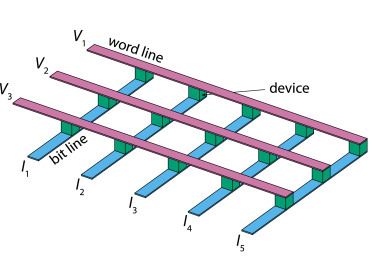
\includegraphics[width=.45\linewidth]{crossbar/crossbar3D.jpg}}\\
  \caption{Memristor crossbar array}
  \label{fig:crossbar}
\end{figure}

It uses physical properties of electrical systems to perform analog computing. In what follows I will use the circuit node in \cref{fig:crossNode} to explain the theory behind the memristor crossbar array.
\begin{figure}[H]
  \centering
  \includesvg[height=3.5cm]{crossbar/node}
  %\def\svgheigth{3.5cm}
  %\input{crossbar/node.pdf_tex}
  \caption{Memristor crossbar node of the $k^{th}$ line and $j^{th}$ column}
  \label{fig:crossNode}
\end{figure}

First of all, a voltage is applied on the $k^{th}$ line, because every column is virtually grounded, the voltage applied to the memristor, of a set resistance $\symR_k$, is $\symv_k$. As such and using Ohm's law, we know that the current flowing into the memristor ($\symi_{k}$) is bound by the following equation :

\begin{equation}
  \symv_k = \symR_k\cdot \symi_{k} \Rightarrow \symi_{k} = \symv_k\cdot (\frac{1}{\symR_k})= \symv_k\cdot \symG_k
\end{equation}
With $\symG_k$ being the conductance of memristor, defined as $\symG_k=\frac{1}{\symR_k}$.

This line then joins the column where a current of $\symi_{j,k-1}$ is flowing, then according to Kirchhoff's current law the resulting current is :
\begin{equation}
  \symi_{j,k} = \symi_{j,k-1}+\symi_{k} = \symi_{j,k-1} + \symv_k\cdot \symG_k
\end{equation}
By applying this process to the whole system we find that the current at the bottom of one column is :
\begin{equation}
  \symi_1= \symG_1\cdot \symv_1 +  \symG_2\cdot \symv_2 +  \symG_3\cdot \symv_3
\end{equation}
With $\symG_1$, $\symG_2$ and $\symG_3$ being the conductance of the 3 memristors in the first column.

Using such an analog circuit is a huge gain in time, for two main reasons :

\begin{itemize}
  \item By being analog, this circuit allows for analog computations which are much faster than their digital counterparts. As explained in this section, the circuit only uses physical properties of the different components and can compute large \acp{VMM} in a very short amount of time.
  \item The other advantage of such a system is the use of the memristors, that make the need to copy data from another memory useless as the memristors have a long term memory themselves. This is one of the ways to break down the Von Neumann bottleneck.
\end{itemize}

\section{Memristor's model}\label{sec:model}

They are several ways to model a memristor \cite{memristorFab,memTEAMmodel, memVTEAMmodel, memristorSpiceModels}. The way the memristor works depends on the materials used to fabricate the memristor. Each type of memristor has slightly different behavior. Models were thus created to simulate, as accurately as possible, the memristor in electrical circuit simulation software such as \textbf{Cadence}'s \textit{virtuoso} or SPICE.

Some examples of memristor's model are :

\begin{itemize}
  \item \acf{LIDM}, the model of the first memristor \cite{memristorFab}.
  \item \acf{STBM}, is another model of the $TiO_x$ memristor created in 2008 by \textbf{HP} \cite{memristorFab, memristorSpiceModels}.
  \item \acf{TEAM}, is a model that can easily adapt to several types of memristive devices while focusing on fast computation \cite{memTEAMmodel}.
  \item \acf{VTEAM}, is a later improvement of the \ac{TEAM}. The internal resistance depends on voltage, unlike \ac{TEAM} which depends on current \cite{memVTEAMmodel}.
\end{itemize}

The \ac{VTEAM} being the most versatile model, its implementation would fit most memristor types.

\subsection{Equations}

It's been established that the internal resistance also depends on an internal state $x$ (\cref{eq:memristiveDev}).

\begin{equation}
  \frac{dx}{dt}=f(x,v)
\end{equation}

Where $v$ is the voltage, $t$ is time and $f$ is a function.

The function $f$ is described in its simplest form as in \cref{eq:funcDesc}.

\begin{equation}\label{eq:funcDesc}
  f(x,v)=g(x)\cdot s(v)
\end{equation}

Where $g$ is the window function and $s$ the sensitivity function.

\begin{itemize}
  \item The window function delimits the operational boundaries of the memristor.
  \item The sensitivity function, also known as voltage sensitivity describes the effect of voltage on the internal state's variations.
\end{itemize}

The model is based on previous work \cite{memCadenceModel} that aims to reproduce as many memristive device types. They have chosen to use the resistive state ($R$) as the internal state \cite{memModelOrigin}. Based on this assumption the \cref{eq:memModel0,eq:memModel1} are extracted from the memristive device. This model is of course very basic and ignores some physical dependencies such as temperature.

\begin{equation}\label{eq:memModel0}
  i(R,v)=
  \begin{cases}
    \frac{a_p}{R}\cdot sinh(b_p\cdot v) & v\ge 0\\
    \frac{a_n}{R}\cdot sinh(b_n\cdot v) & v<0\\
  \end{cases}
\end{equation}

\begin{equation}\label{eq:memModel1}
  \frac{dR}{dt}=f(R,v)=s(v)\cdot g(R,v)
\end{equation}

The sensitivity function was chosen to be a voltage-dependent exponential function, like described in \cref{eq:memModel2}.

\begin{equation}\label{eq:memModel2}
  s(v)=
  \begin{cases}
    A_p\cdot (e^{t_p\cdot |v|}-1)& v>0\\
    A_n\cdot (e^{t_n\cdot |v|}-1)& v<0\\
    0 &  v=0\\
  \end{cases}
\end{equation}

The window function used is a state-dependent quadratic function as shown in \cref{eq:memModel3}.

\begin{equation}\label{eq:memModel3}
  g(R,v)=
  \begin{cases}
    (R-r_p(v))^2& v>0\\
    (R-r_n(v))^2& v<0\\
    0 &  v=0\\
  \end{cases}
\end{equation}

Where $r_p$ and $r_n$ are voltage dependent in a polynomial manner. They represent the boundaries of the state variable. All the other parameters in \cref{eq:memModel0,eq:memModel1,eq:memModel2,eq:memModel3} that haven't been declared are free fitting variables. They have to be set depending on the type of memristor used.

\subsection{Verilog-A integration}

The model now needs to be adapted to work as Verilog-A code.
Verilog-A is a hardware desciption language, very popular in the industry for its simplicity and flexibility when using it with circuit simulator such as \textbf{Cadence}'s \textit{virtuoso}.

The focus of this specific implementation will be the resistance range $[20k\Omega, 120k\Omega]$. The boundaries functions are found in \cref{eq:memModel4}.

\begin{equation}\label{eq:memModel4}
  \begin{cases}
    r_p(v)= r_{p,0} + r_{p,1}\cdot v& v>0\\
    r_n(v)= r_{r,0} + r_{n,1}\cdot v& v\le 0\\
  \end{cases}
\end{equation}

Where $r_{p,0}$, $r_{p,1}$, $r_{n,0}$ and $r_{n,1}$ are free fitting variables that need to be extracted from the physical device.

The changes of resistive states from the initial resistance ($R_0$) are computed by \cref{eq:memModel5} extracted from \cite{memCadenceModel}. It uses the bias voltage ($V_b$) of the pulse applied to the memristor. The pulse has a duration of $t$.

\begin{equation}\label{eq:memModel5}
  R(t)_{|V_b} =
  \begin{cases}
    \frac{R_0+s(V_b)\cdot r_p(V_b)\cdot(r_p(V_b)-R_0)\cdot t}{1+s(V_b)\cdot (r_p(V_b)-R_0)\cdot t} & V_b>0, R<r_p(V_b)\\
    \frac{R_0+s(V_b)\cdot r_n(V_b)\cdot(r_n(V_b)-R_0)\cdot t}{1+s(V_b)\cdot (r_n(V_b)-R_0)\cdot t} & V_b\le 0, R>r_n(V_b)\\
    R_0 & else\\
  \end{cases}
\end{equation}

The final Verilog-A code is available at \cref{apsec:memModel}.

\subsection{Behavior}

The model was tested then tested. As with physical memristors, it has a threshold voltage value from which its resistive states starts changing. This threshold value is $V_{read}$. For this specific model the threshold voltage is set to $V_{read}=500mV$.

Every pulse is composed of 2 parts and last for a total of $1 ms$ :
\begin{itemize}
  \item The reading of the resistive state, by applying a triangular wave that in bound by the threshold value $V_{read}$.
  \item The writing to the memristor. During this part the resistive state will change. This is done by apply a square wave of variable width ($t_{\Delta}$) with a set bias voltage ($V_{bias}$).
\end{itemize}

\begin{figure}[H]
  \centering
  \includesvg[width=\textwidth]{memristor/input.svg}
  \label{graph:memInput}
  \caption{Pulse shape graph}
\end{figure}

The \cref{graph:memInput} is the visual representation of what each pulse, the value is read during the first half of the pulse.

The resistive state of the memristor changes depending on the pulse width ($t_{\Delta}$) and the bias voltage ($V_{bias}$) used for each pulse.

\begin{figure}[H]
  \centering
  \includesvg[width=\textwidth]{memristor/memPulseChange.svg}
  \label{graph:pulseChange}
  \caption{Memristor's resistive state under different pulses width (Fixed bias voltage $V_{bias}=1.8V$)}
\end{figure}

The effect of the pulse width variation is shown in \cref{graph:pulseChange}. Indeed, the larger the pulse widths, the faster the internal resistance reaches the bounding resistance (\cref{eq:memModel4}). The bounding resistance being the same as all curve use the same bias voltage ($V_{bias}=1.8V$), the curves will all eventually reach the max resistance.

\begin{figure}[H]
  \centering
  \includesvg[width=\textwidth]{memristor/memVoltChange.svg}
  \label{graph:voltChange}
  \caption{Memristor's resistive state under different voltages (Fixed pulse width $t_{\Delta}=100\mu s$)}
\end{figure}

The voltage dependence of the memristor's model is described in \cref{graph:voltChange}. The influence of the bias voltage is, as \cref{eq:memModel3,eq:memModel4} show, the way to change the resistance range of the memristor, until the physical limit is reached of course. Applying higher voltage also allows to reach a set resistance faster as the slopes are bigger the higher the bias voltage gets.

The resistive state can also be lowered by applying negative voltages.TODO

%\subsection{\acf{LIDM}}

%The \ac{LIDM} is the model of the first memristor eveer created, it was created to fit the behavior of the $TiO_x$ memristor they had just fabricated \cite{memristorFab}. The device, of width $D$, has two parts. The doped part and the undoped


\cleardoublepage
